% asset_id: AS2ModellingInMechanicsTIKZ-002
\documentclass[tikz,border=8pt]{standalone}
\usepackage{amsmath}
\usetikzlibrary{arrows.meta, positioning}
\begin{document}
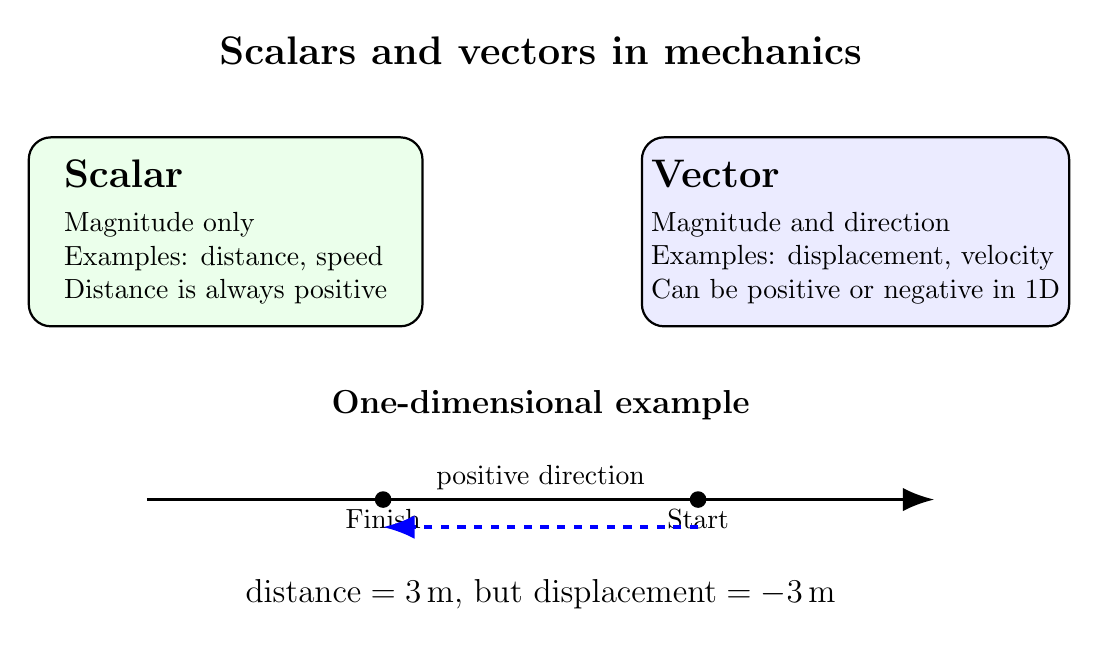
\begin{tikzpicture}[card/.style={draw, rounded corners=8pt, thick, minimum width=5cm, minimum height=2.4cm, align=left}, arrow/.style={-{Latex[length=4mm]}, very thick}]
\node[font=\Large\bfseries] at (0,3.7) {Scalars and vectors in mechanics};
\node[card, fill=green!8] at (-4,1.4) {\Large\textbf{Scalar}\\[4pt]Magnitude only\\Examples: distance, speed\\Distance is always positive};
\node[card, fill=blue!8] at (4,1.4) {\Large\textbf{Vector}\\[4pt]Magnitude and direction\\Examples: displacement, velocity\\Can be positive or negative in 1D};
\node[font=\large\bfseries] at (0,-0.8) {One-dimensional example};
\draw[arrow] (-5,-2) -- (5,-2);\node[above] at (0,-2) {positive direction};
\fill (-2,-2) circle (3pt);\node[below] at (-2,-2) {Finish};\fill (2,-2) circle (3pt);\node[below] at (2,-2) {Start};
\draw[-{Latex[length=4mm]}, dashed, very thick, blue] (2,-2.35) -- (-2,-2.35);
\node[font=\large] at (0,-3.2) {$\text{distance}=3\,\mathrm{m}$, but $\text{displacement}=-3\,\mathrm{m}$};
\end{tikzpicture}
\end{document}
